\begin{figure*}
\centering
    \begin{subfigure}{0.1\textwidth}
	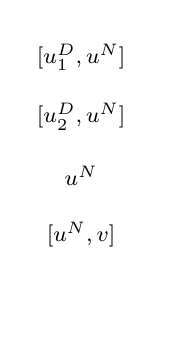
\begin{tikzpicture}
	    \begin{scope}[scale=0.75]
		\node at (0,0.5) {\footnotesize $\T{[u^N,v]}$};
		\node at (0,1.5) {\footnotesize $\R{u^N}$};
		\node at (0,2.5) {\footnotesize $\T{[u_2^D, u^N]}$};
		\node at (0,3.5) {\footnotesize $\T{[u_1^D, u^N]}$};
		\draw[white] (0,4)--(1,4);
		\draw[white] (0,-0.8)--(1,-0.8);
	    \end{scope}
	\end{tikzpicture}
    \end{subfigure}
    \begin{subfigure}{0.25\textwidth}
	\centering
	\begin{tikzpicture}
	    \begin{scope}[scale=0.75]
		\draw[thick] (0,0) -- (5,0);
		\draw[thick] (0,1) -- (5,1);
		\draw[thick] (0,2) -- (5,2);
		\draw[thick] (0,3) -- (5,3);
		\draw[thick] (0,4) -- (5,4);

		\draw[pattern=north east lines] (0.5,3) rectangle ++(2,0.7);
		\draw[fill=black!20] (1,3) rectangle ++(1.3,0.6) node[pos=.5] {$f_1$};
		\draw[<-, thick] (0.5,3.9) -- (0.5,3);

		\draw[pattern=north west lines] (1,2) rectangle ++(2,0.7);
		\draw[fill=black!20] (1,2) rectangle ++(1.8,0.6) node[pos=.5] {$f_2$};
		\draw[<-, thick] (1,2.9) -- (1,2);

		\draw[pattern=north east lines] (1.5,1) rectangle ++(1,0.7);
		\draw[pattern=north west lines] (2,1) rectangle ++(1,0.7);

		\draw[pattern=north west lines] (2.5,0) rectangle ++(2,0.7);
		\draw[pattern=north east lines] (2.5,0) rectangle ++(2,0.7);
		\draw[fill=black!20] (2.5,0) rectangle ++(1,0.6) node[pos=.5] {$f_2$};
		\draw[fill=black!20] (3.2,0) rectangle ++(1,0.6) node[pos=.5] {$f_1$};
	    \end{scope}
	\end{tikzpicture}
      \caption{Basic Consistency} \label{fig:exec_seq:basic_consistency}
    \end{subfigure}
    \begin{subfigure}{0.25\textwidth}
	\centering
	\begin{tikzpicture}
	    \begin{scope}[scale=0.75]
		\draw[thick] (0,0) -- (5,0);
		\draw[thick] (0,1) -- (5,1);
		\draw[thick] (0,2) -- (5,2);
		\draw[thick] (0,3) -- (5,3);
		\draw[thick] (0,4) -- (5,4);

		\draw[pattern=north east lines] (0.5,3) rectangle ++(2,0.7);
		\draw[fill=black!20] (0.5,3) rectangle ++(1.3,0.6) node[pos=.5] {$f_1$};
		\draw[<-, thick] (0.5,3.9) -- (0.5,3);

		\draw[pattern=north west lines] (1,2) rectangle ++(2,0.7);
		\draw[fill=black!20] (1,2) rectangle ++(1.8,0.6) node[pos=.5] {$f_2$};
		\draw[<-, thick] (1,2.9) -- (1,2);

		\draw[pattern=north east lines] (1.5,1) rectangle ++(1,0.7);
		\draw[pattern=north west lines] (2,1) rectangle ++(1,0.7);

		\draw[pattern=north west lines] (2.5,0) rectangle ++(2,0.7);
		\draw[pattern=north east lines] (2.5,0) rectangle ++(2,0.7);
		\draw[fill=black!20] (2,0) rectangle ++(1,0.6) node[pos=.5] {$f_1$};
		\draw[fill=black!20] (3.5,0) rectangle ++(1,0.6) node[pos=.5] {$f_2$};
	    \end{scope}
	\end{tikzpicture}
	\caption{GCL Consistency} \label{fig:exec_seq:gcl_consistency}
    \end{subfigure}
    \begin{subfigure}{0.25\textwidth}
	\centering
	\begin{tikzpicture}
	    \begin{scope}[scale=0.75]
		\draw[thick] (0,0) -- (5,0);
		\draw[thick] (0,1) -- (5,1);
		\draw[thick] (0,2) -- (5,2);
		\draw[thick] (0,3) -- (5,3);
		\draw[thick] (0,4) -- (5,4);

		\draw[pattern=north east lines] (0.5,3) rectangle ++(2,0.7);
		\draw[fill=black!20] (0.5,3) rectangle ++(1.5,0.6) node[pos=.5] {$f_1$};
		\draw[<-, thick] (0.5,3.9) -- (0.5,3);

		\draw[pattern=north west lines] (1,2) rectangle ++(2,0.7);
		\draw[fill=black!20] (1,2) rectangle ++(2,0.6) node[pos=.5] {$f_2$};
		\draw[<-, thick] (1,2.9) -- (1,2);

		\err at (3,2);

		\draw[pattern=north east lines] (1.5,1) rectangle ++(1,0.7);
		\draw[pattern=north west lines] (2,1) rectangle ++(1,0.7);

		\draw[pattern=north west lines] (2.5,0) rectangle ++(2,0.7);
		\draw[pattern=north east lines] (2.5,0) rectangle ++(2,0.7);
		\draw[fill=black!20] (3,0) rectangle ++(1,0.6) node[pos=.5] {$f_2$};
	    \end{scope}
	\end{tikzpicture}
	\caption{Stream Policing} \label{fig:exec_seq:stream_policing}
    \end{subfigure}
    \caption{Invalid execution sequences violating Basic Consistency (a), GCL Consistency (b), or Stream Policing (c)}
    \label{fig:exec_seq}
\end{figure*}


\subsection{Formal Definition of Execution Sequences}
For a network graph $G$ with TSN configuration $\Conf = (\R{}, \GCL{})$, we define an execution sequence $\E(G, \C)$ as a tuple $(\T{}, \D{})$,\footnote{If both $G$ and $\Conf$ are clear from context, we simply write $\E$.} where, for each link $[u,v] \in E$ and frame $f \in \TT_{[u,v]}$
\begin{itemize}
    \item $\T{[u,v],f}$ describes the transmission offset in $\E$, and
    \item $\D{[u,v],f}$ describes the transmission delay in $\E$.
\end{itemize}
To model dropped frames, an execution sequence is allowed to assign $\infty$ to $\T{}$ and $\D{}$.

Formalizing execution sequences is motivated by two aspects.
First, formal constraints are required to prove robustness of a TSN configuration $\Conf$.
Second, formal constraints provide valuable insight into the technical requirements the network infrastructure must provide to guarantee the services' reliability requirements.
We start in Section~\ref{sec:execution_sequences:notation} with notational conventions.
Thereafter, the constraints \textit{Basic Consistency}, \textit{GCL Consistency}, and \textit{Stream Policing} are introduced.
To illustrate the effects and the importance of each constraint, we refer to Fig.~\ref{fig:exec_seq} throughout these sections.

\subsubsection{Notational Conventions}\label{sec:execution_sequences:notation}
An execution sequence $\E$ specifies the transmission offsets $\T{}$ and the transmission delays $\D{}$. 
To model dropped frames of a TSN stream $f \in \TT$, we allow $\T{}$ and $\D{}$ to map to $\infty$, conveying the following semantics:
\begin{enumerate}[label=I\arabic*)]
  \item If $\T{[\v{k}{f}, \v{k+1}{f}],f} < \infty$ but $\D{[\v{k}{f}, \v{k+1}{f}],f} = \infty$, $f$ is dropped by $\v{k}{f}$ during its transmission over $[\v{k}{f}, \v{k+1}{f}]$.
  \item If $\D{[\v{k}{f}, \v{k+1}{f}],f} < \infty$ but $\T{[\v{k+1}{f}, \v{k+2}{f}],f} = \infty$, $f$ is dropped by $\v{k+1}{f}$ upon receipt.
\end{enumerate}

While $\D{[\v{k}{f}, \v{k+1}{f}],f} = \infty$ and I1 capture the message streams' view, we also require a formalism that tells $\v{k}{f}$ when it is allowed to start the transmission of the subsequent frame.\footnote{In fluid dynamics, these two points of view correspond to the Lagrangian and Eulerian observers, respectively.}
For this purpose, we define the \textit{effective} transmission delay $\eD{}$ to be equal to the upper PDB bound $\dpdbmax{}$, if I1 occurs, i.e.,
\begin{equation}\label{eq:eD}
  \eD{[\v{k}{f}, \v{k+1}{f}],f} = \begin{cases}
    \dpdbmax{[\v{k}{f}, \v{k+1}{f}],f} \quad &\text{for } \text{I1}, \\
    \D{[\v{k}{f}, \v{k+1}{f}],f} \quad &\text{else.}
    \end{cases}
\end{equation}


\subsubsection{Basic Consistency} \label{sec:execution_sequences:basic_consistency}
Basic Consistency restrains the execution sequence $\E$ to ensure mutual exclusion of transmission links (i.e., Ethernet links and 5G frequency channels), sequential transmission, isochronous talkers, and FIFO queuing.

\textbf{\TC} \label{sec:execution_sequences:basic_consistency:tc}
ensures that for every link $[u,v] \in E$, no two frames $f, f' \in \TT_{[u,v]}$ with $f \neq f'$ transmit at the same time, i.e.,
\begin{align*}
  \add{\T}{\eDtrans}{[u,v], f} &\leq \T{[u,v], f'}, \qquad \text{or}\\
  \add{\T}{\eDtrans}{[u,v], f'} &\leq \T{[u,v], f}.
\end{align*}
Fig.~\ref{fig:exec_seq:basic_consistency} violates this constraint by overlapping the transmission of frames $f_1$ and $f_2$ at $[u^N, v]$.

\textbf{\ST} \label{sec:execution_sequences:basic_consistency:st}
ensures that for every stream $f \in \TT$ and every $1 \leq k < n(f)$ that the transmission of $f$ over $[\v{k}{f}, \v{k+1}{f}]$ can only start after $f$ is fully received by $\v{k}{f}$, i.e.,
\begin{equation*}
  \add{\T}{\D}{[\v{k}{f}, \v{k+1}{f}], f} \leq \T{[\v{k+1}{f}, \v{k+2}{f}], f}.
\end{equation*}
Fig.~\ref{fig:exec_seq:basic_consistency} violates this constraint by starting the transmission of $f_2$ at $[u^N, v]$ before $f_2$'s transmission over $[u^D_2, u^N]$ completed.

\textbf{$\IT$} \label{sec:execution_sequences:basic_consistency:it}
ensures that for every stream $f \in \TT$ that the talker $\v{1}{f}$ starts its transmission as configured 
\begin{equation*}
  \T{[\v{1}{f}, \v{2}{f}], f} = \Smin{[\v{1}{f}, \v{2}{f}], f}.
\end{equation*}
Fig.~\ref{fig:exec_seq:basic_consistency} violates this constraint by starting the transmission of $f_1$ at $[u_1^D, u^N]$ too late.

\textbf{$\FIFO$} \label{sec:execution_sequences:basic_consistency:fifo}
ensures that for every link $[v,w] \in E$ and every two frames $f, f' \in \TT_{[v,w]}$, with respective previous hops $[u,v]$ and $[u',v]$, that the transmission order is identical to the receiving order, i.e,
\begin{align*}
  \add{\T}{\D}{[u,v], f} < \add{\T}{\D}{[u',v], f'} \\
    \iff \T{[v,w], f} < \T{[v,w], f'}.
\end{align*}
Fig.~\ref{fig:exec_seq:basic_consistency} violates this constraint by transmitting $f_2$ over $[u^N, v]$ before $f_1$, whereas $f_1$ arrives at $u^N$ before $f_2$.

\subsubsection{GCL Consistency}\label{sec:execution_sequences:gcl}
GCL Consistency restrains the execution sequence $\E$ to respect the configured GCL $\GCL([v,w])$ for every link $[v,w] \in E$.
For this purpose, let
\begin{equation*}
    \GCL([v,w]) = [(o_1,c_1), \ldots, (o_m,c_m)].
\end{equation*}
GCL Consistency consists of encapsulation and progress.

\textbf{$\GCLC$} \label{sec:execution_sequence:gcl:completeness}
ensures for every arrived frame $f \in \TT_{[v,w]}$, i.e., $\T{[v,w],f} < \infty$, that $v$ transmits $f$ within a configured window $(o_i, c_i)$, i.e.,
\begin{equation}\label{eq:gclc}
    o_i \leq \T{[v,w], f} \leq c_i - \dpdbtransmax{[v,w], f}.
\end{equation}
Fig.~\ref{fig:exec_seq:gcl_consistency} violates this constraint by starting the transmission of $f_1$ at $[u^N, v]$ before the gate opens.

\textbf{$\GCLS$}\label{sec:execution_sequence:gcl:soundness}
ensures for every transmission window $(o_i, c_i)$ and every point in time $o_i \leq t < c_i$ that, if the queue at $[v,w]$ is not empty, i.e., there exists a frame $f \in \TT_{[v,w]}$ with previous hop $[u,v]$ and
\begin{equation*}
  \add{\T}{\D}{[u,v], f} \leq t \leq \T{[v,w], f} < \infty, 
\end{equation*}
there exists $f' \in \TT_{[v,w]}$, potentially different from $f$, which is transmitting over $[v,w]$ at time $t$, i.e.,
\begin{equation*}
  \T{[v,w], f'} \leq t < \add{\T}{\eDtrans}{[v,w], f'}. 
\end{equation*}
Fig.~\ref{fig:exec_seq:gcl_consistency} violates this constraint by having a gap between $f_1$'s and $f_2$'s transmission at $[u^N, v]$, although the gate remains open and $f_2$ arrives at $u^N$ before $f_1$'s transmission finishes.

\subsubsection{Stream Policing} \label{sec:execution_sequences:stream_policing}
Stream Policing restrains the execution sequence $\E$ to drop frames correctly. 
There are two important aspects that have to be covered to correctly model wireless TSN behavior.
First, a frame is dropped by a TSN bridge if it
\begin{enumerate}[label=I\arabic*)]
  \item transmits longer than the PDB $\dpdb{}$, or
    \item arrives outside the PSFP interval.
\end{enumerate}
Second, $\E$ cannot drop frames arbitrarily, that is, if a frame is dropped, it must be because of I1 or I2.

\textbf{$\TP$}
ensures for every stream $f \in \TT$ that $f$ is discarded during transmission over $[\v{k}{f}, \v{k+1}{f}]$ if and only if the transmission duration takes longer than the PDB, i.e.,
\begin{align*}
  \Dtrans{[\v{k}{f}, \v{k+1}{f}],f} > \dpdbtransmax{[\v{k}{f}, \v{k+1}{f}],f} \\
    \iff \Dtrans{\clink{k}{f},f} = \infty.
\end{align*}
Fig.~\ref{fig:exec_seq:stream_policing} shows this behavior by dropping $f_2$ at $[u_2^D, u^N]$, i.e., $\Dtrans{[u_2^D, u^N], f_2} = \infty$, as indicated by the cross, after its transmission is not successfully completed within its PDB.

\textbf{$\PSFP$}
ensures for every stream $f \in \TT$ that $f$ is dropped by PSFP at $\v{k}{f}$ ($k > 1$), if and only if it arrives outside the PSPF interval, i.e.,
\begin{align*}
  \add{\T}{\D}{\pclink{k}{f},f} \notin \R{\v{k}{f},f} \\
    \iff \T{\clink{k}{f},f} = \infty.
\end{align*}
Fig.~\ref{fig:exec_seq:stream_policing} violates this constraint by dropping $f_1$ at $u^N$, i.e., $\T{[u^N, v], f_1} = \infty$, although it arrived within the PSFP interval.

\textbf{$\PC$}
is used for consistent modelling of the execution sequence $\E$, ensuring that once a frame is dropped, it remains dropped for all subsequent hops.
Thus, we require for every stream $f \in \TT$ and every hop $\clink{k}{f}$ that
\begin{equation} \label{eq:pc:1}
  \T{\clink{k}{f},f} = \infty \implies \D{\clink{k}{f},f} = \infty.
\end{equation}
Further, we require $\clink{k}{f}$ with $k < n - 1$ to satisfy
\begin{equation} \label{eq:pc:2}
  \D{\clink{k}{f},f} = \infty \implies \T{\nclink{k}{f},f} = \infty.
\end{equation}
While (\ref{eq:pc:2}) would also be satisfied by combining (\ref{eq:pc:1}) with $\textsf{PSFP}$ or $\textsf{SequentialTransmission}$, we prefer an explicit separation of constraint functionality.
Fig.~\ref{fig:exec_seq:stream_policing} violates this constraint by transmitting $f_2$ over $[u^N, v]$, i.e., $\T{[u^N, v], f_2} < \infty$, although it was previously dropped by $\TP$ during its transmission at $[u_2^D, u^N]$.

\subsection{Proof of Theorem~\ref{theorem:feasibility}} \label{appendix:feasibility}
By allocating sufficiently large 5G PDBs to satisfy~(\ref{eq:pdb2}) for stream $F$, the following holds true for all frames $f \in F$:
\begin{align}
  &\rel{F} \leq \prod_{[u,v] \in \path{F}} \Prob\big(\D{[u,v], f} \in \dpdb{[u,v], f}\big) \\
  = &\sum_{\E} \prod_{[u,v]} \Prob\big(\D{[u,v], f} \in \dpdb{[u,v], f} \mid \E \big) \times \Prob(\E), \label{eq:ap1}
\end{align}
By Definition~\ref{def:robustness}, the arrival time $A(f)$ is within the expected interval $\R{\vl{F}, f}$ if all packet delays along $\path{F}$ lie within their respective PDBs.
We can write 
\begin{align*}
  (\ref{eq:ap1}) &\leq \sum_{\E} \Prob\big(A(f) \in \R{\vl{F}, f} \mid \E\big) \times \Prob(\E) \\
   &= \Prob\big(A(f) \in \R{\vl{F}, f}\big).
\end{align*}
Hence, the probability of $f$ arriving within $\R{\vl{F}, f}$ exceeds the required $\rel{F}$.
Also, (iii) of Theorem~\ref{theorem:feasibility} constrains $\R{\vl{F}, f}$ to satisfy the latency and jitter bounds of $F$.

\subsection{Proof of Theorem~\ref{theorem:fips_robust}} \label{appendix:theorem_proof}
We start with some notational conventions:
First, compared to $\S{[u,v], B_i}$, which defines the transmission start of a frame batch at $[u,v]$, we want to verify when a frame $f \in B_i$ can start its transmission.
We therefore define the interval $\S{} = [\Smin{}, \Smax{}]$ to capture the (intended) minimum and maximum transmission times, i.e.,
\begin{align} \label{eq:sminmax}
  \Smin{[u,v], f} = \S{[u,v], B_i} \quad \text{and} \quad \Smax{[u,v], f} = \sum_{f' \in B_i \setminus \{f\}} \dpdbtransmax{[u,v], f'},
\end{align}
for each $[u,v] \in E$ and $f \in \TT_{[u,v]}$.
Here, $\dpdbtransmax{}$ solely captures the serialization delay (for both Ethernet links and 5G links).
Moreover, to have a clear mapping between frames $f$ and their corresponding batch, we write $\I{[u,v], f} = B_i$.

Given an execution sequence $\E = (\T{}, \D{})$, we define $\S{}^\E$ as the \textit{expected transmission offset for $\E$} with
\begin{equation} \label{eq:fips:se}
  \S{}^\E([u,v],f) = \Smin{[u,v],f} + \sum_{f' \in B^\E([u,v], f)} \eDtrans{[u,v],f'},
\end{equation}
for $[u,v] \in E$ and $f \in \TT_{[u,v]}$, where $B^\E([u,v], f)$ denotes frames $f' \in B([u,v], f)$ which are transmitted over $[u,v]$ before $f$, i.e., $\T{[u,v],f'} < \T{[u,v],f}$.
We commence with structured proofs to show the robustness of FIPS.

\begin{lemma}\label{lemma:fips:aux}
  Let $\S{}$ denote a schedule that concurs with FIPS, and $\Conf$ the derived FIPS configuration. 
  Then, for every execution sequence $\E = (\T{}, \D{})$ we have $\S{}^\E([u,v],f) \in \S{[u,v],f}$, for all $[u,v] \in E$ and $f \in \TT_{[u,v]}$.
\end{lemma}
\begin{proof}
    \textit{Proof:}
    \pflet{$[u,v] \in E$ and $f \in \TT_{[u,v]}$}
    \step{<2>1}{$\SE{[u,v],f} \geq \Smin{[u,v],f}$}
    \begin{proof}
      \pf\ By definition of $\SE{[u,v],f}$ in (\ref{eq:fips:se}).
    \end{proof}
    \step{<2>2}{$\SE{[u,v],f} \leq \Smax{[u,v],f}$}
    \begin{proof}
      \step{<3>1}{$\IE{[u,v], f} \subseteq \I{[u,v], f} \backslash \{f\}$}
	\begin{proof}
	    \pf\ By definition of $\IE{[u,v], f}$.
	\end{proof}
	\step{<3>2}{$\eDtrans{[u,v],f'} \leq \dpdbtransmax{[u,v],f'}$ for all $f' \in \IE{[u,v],f}$}
	\begin{proof}
	    \step{<4>1}{$\T{[u,v], f'} < \infty$}
	    \begin{proof}
		\pf\ By definition of $\IE{[u,v], f'}$, we have $\T{[u,v], f'} < \T{[u,v], f}$
	    \end{proof}
	    \step{<4>2}{\case{$\Dtrans{[u,v],f'} = \infty$}}
	    \begin{proof}
		\pf\ $\eDtrans{[u,v],f'} = \dpdbtransmax{[u,v], f'}$ by (\ref{eq:eD}) with case assumption \stepref{<4>2} and step \stepref{<4>1}.
	    \end{proof}
	    \step{<4>3}{\case{$\Dtrans{[u,v],f'} < \infty$}}
	    \begin{proof}
		\step{<5>1}{$\eDtrans{[u,v],f'} = \Dtrans{[u,v],f'}$}
		\begin{proof}
		    \pf\ By definition of $\eD{[u,v],f'}$ in (\ref{eq:eD}) with case assumption \stepref{<4>3}.
		\end{proof}
		\step{<5>2}{$\Dtrans{[u,v],f'} \leq \dpdbtransmax{[u,v],f'}$}
		\begin{proof}
		    \pf\ By $\TP$ and case assumption \stepref{<4>3}.
		\end{proof}
		\qedstep
		\begin{proof}
		    \pf\ By steps \stepref{<5>1} and \stepref{<5>2}.
		\end{proof}
	    \end{proof}
	\end{proof}
	\qedstep
	\begin{proof}
	    \pf\ By steps \stepref{<3>1}, \stepref{<3>2}, we have
	    \begin{align*}
	      \SE{[u,v],f} \leq \Smin{[u,v],f} + \sum_{f' \in \I{[u,v], f} \backslash \{f\}} \dpdbtransmax{[u,v],f'} = \Smax{[u,v],f}
	    \end{align*}
	\end{proof}
    \end{proof}
    \qedstep
    \begin{proof}
	\pf\ By steps \stepref{<2>1} and \stepref{<2>2}. 
    \end{proof}
\end{proof}

\begin{lemma}\label{lemma:fips}
  Let $\S{}$ denote a schedule that concurs with FIPS, and $\Conf$ the derived FIPS configuration. 
    Then, for every execution sequence $\E = (\T{}, \D{})$ and every message stream $f \in \TT$, the following holds true:
    For $1 \leq l < n(f)$, if $f$ arrives at $\v{l}{f}$ within its PSFP enforced interval, i.e.,
    \begin{equation*}
      \add{\T}{\D}{\pclink{l}{f},f} \in \R{\v{l}{f},f},
    \end{equation*}
    then $\v{l}{f}$ starts the transmission of $f$ as expected by $\S{}^\E$, i.e.,
    \begin{equation*}
      \T{\clink{l}{f},f} = \SE{\clink{l}{f},f}.
    \end{equation*}
\end{lemma}
\begin{proof}
    \textit{Proof:}
    \define{$\V \subseteq E \times \TT$ with $(\clink{l}{f},f) \in \V$, if and only if
	\begin{pfenum}
	\item $\add{\T}{\D}{\pclink{l}{f},f} \in \R{\v{l}{f}, f}$, and
	\item  $\T{\clink{l}{f}, f} \neq \SE{\clink{l}{f}, f}$.
	\end{pfenum}
    }
    \assume{$\V \neq \emptyset$}
    \prove{False}
    \explan{Proof by contradiction.
	Assume $\V \neq \emptyset$ and pick $(\clink{l}{f},f) \in \V$ which is the ``first'' to deviate from the expected transmission offset (step \estepref{1}{1}).
	There are three possible cases to consider: 
	\begin{itemize}
	  \item Step \estepref{1}{4}: the frame $f$ starts its transmission too late, i.e., after $\SE{\clink{l}{f},f} < \T{\clink{l}{f},f}$,
	  \item Step \estepref{1}{5}: the frame $f$ starts its transmission too soon but still within $\S{\clink{l}{f},f}$, i.e., $\Smin{\clink{l}{f},f} \leq \T{\clink{l}{f},f} < \SE{\clink{l}{f},f}$, or
	  \item Step \estepref{1}{6}: the frame $f$ starts its transmission too soon and even before $\Smin{\clink{l}{f},f}$, i.e., $\T{\clink{l}{f},f} < \Smin{\clink{l}{f},f}$.
	\end{itemize}
	We derive a contradiction for each case.
    }
    \pflet{$\GCL(\clink{l}{f}) = [(o_1, c_1), \ldots, (o_m, c_m)]$}
    \step{<1>1}{\pick{ $(\clink{l}{f},f) \in \V$ with $\T{\clink{l},f}$ minimal}}
    \begin{proof}
        \pf\ Exists by assumption {\toplevel} and since $\V \subseteq E \times \TT$ is finite.
    \end{proof}
    \step{<1>3}{$\T{\clink{l}{f},f} < \infty$}
    \begin{proof}
	\pf\ By $\PSFP$ with step \stepref{<1>1} and definition \toplevel:1.
    \end{proof}
    \step{<1>4}{\pick{ $1 \leq i \leq m$ with $o_i = \Smin{\clink{l}{f},f}$}}
    \begin{proof}
	\pf\ Exists by construction of FIPS's GCL encoding.
    \end{proof}
    \step{<1>5}{\case{$\SE{\clink{l}{f},f} < \T{\clink{l}{f},f}$}}
    \begin{proof}
      \explan{In case the frame $f$ starts its transmission later than expected, we show that there must be some other frame $f'$ that is still transmitting over $\clink{l}{f}$ at time $\SE{\clink{l}{f},f}$ (step \estepref{2}{1}). 
	    We derive that $f'$ must also start its transmission later than expected (step \estepref{2}{4}), as otherwise its transmission would be aborted before $\SE{\clink{l}{f},f}$.
	    This, however, yields a contradiction to $\T{\clink{l}{f},f}$ being minimal (step \estepref{2}{5}).
        }
	\step{<2>1}{\pick{ $f' \in \TT_{\clink{l}{f}}$, with $f \neq f'$, such that $f'$ is still transmitting over $\clink{l}{f}$ at time $\SE{\clink{l},f}$, i.e., 
        \begin{align*}
	  \T{\clink{l}{f}, f'} \leq \SE{\clink{l}{f},f} < \add{\T}{\eDtrans}{\clink{l}{f}, f'}. 
        \end{align*}
        }}
        \begin{proof}
            \explan{
                The existence of $f'$ follows by $\GCLS$. 
                We therefore have to verify that its precondition is fulfilled.
                On the other hand, $f' \neq f$ as otherwise $f$ would not be delayed.
            }
	    \step{<3>1}{The egress queue at $\clink{l}{f}$ is not empty at time $\SE{\clink{l}{f},f}$, i.e.,
            \begin{align*}
	      \add{\T}{\D}{\pclink{l}{f}, f} \leq \SE{\clink{l}{f},f} \leq \T{\clink{l}{f}, f} < \infty
            \end{align*}}
            \begin{proof}
                \explan{We derive the inequality step by step.}
		\step{<4>1}{$\add{\T}{\D}{\pclink{l}{f}, f} \leq \Rmax{\v{l}{f}, f}$} 
                \begin{proof}
                    \pf\ By step \stepref{<1>1} and definition \toplevel:1.
                \end{proof}
		\step{<4>2}{$\Rmax{\v{l}{f}, f} \leq \Smin{\clink{l}{f},f}$} 
                \begin{proof}
                    \pf\ By C1.
                \end{proof}
		\step{<4>3}{$\Smin{\clink{l}{f}, f} \leq \SE{\clink{l}{f},f}$} 
                \begin{proof}
                    \pf\ By Lemma~\ref{lemma:fips:aux}.
                \end{proof}
                \qedstep
                \begin{proof}
                    \pf\ By steps \stepref{<4>1}, \stepref{<4>2}, \stepref{<4>3}, \stepref{<1>5} (case assumption), and \stepref{<1>3}, in that order.
                \end{proof}
            \end{proof}
            \qedstep
            \begin{proof}
                \pf\ $f'$ exists by $\GCLS$ with step \stepref{<3>1}.
		We have $f' \neq f$, since $\T{\clink{l}{f}, f'} \leq \SE{\clink{l}{f}, f} < \T{\clink{l}{f}, f}$ by case assumption \stepref{<1>5}.
            \end{proof}
        \end{proof}
	\pflet{$l'$ with $\v{l}{f} = \v{l'}{f'}$.}
	\step{<2>2}{$\add{\T}{\D}{\pclink{l'}{f'},f'} \in \R{\v{l}{f}, f'}$}
        \begin{proof}
	  \pf\ By $\PSFP$ with $\T{\clink{l}{f},f'} < \infty$ by step \stepref{<2>1}.
        \end{proof}
	\step{<2>3}{$\add{\SE}{\eDtrans}{\clink{l}{f}, f'} \leq \SE{\clink{l}{f}, f}$}
        \begin{proof}
            \explan{The proof of this inequality depends on whether $f$ and $f'$ are allowed to interleave.}
	    \step{<3>1}{\case{$f' \in \I{\clink{l}{f},f}$}}
            \begin{proof}
	      \explan{If $f$ and $f'$ are allowed to interleave, the inequality directly follows from the definition of $\IE{}$ and $\SE{}$.}
		\step{<4>1}{$f' \in \IE{\clink{l}{f},f}$}
        	\begin{proof}
		  \pf\ $\T{\clink{l}{f},f'} < \T{\clink{l}{f},f}$ by step \stepref{<2>1} and case assumption \stepref{<1>4}.
        	\end{proof}
        	\qedstep
        	\begin{proof}
		  \pf\ The inequality \stepref{<2>3} holds by step \stepref{<4>1} and definition of $\SE{}$ in (\ref{eq:fips:se}).
        	\end{proof}
            \end{proof}
	    \step{<3>2}{\case{$f' \notin \I{\clink{l}{f},f}$}}
            \begin{proof}
                \explan{If $f$ and $f'$ are strictly separated, we highly depend on C3 to yield the inequality \stepref{<2>3}.
                We show the inequality step by step.}
		\step{<4>1}{$\add{\SE}{\eDtrans}{\clink{l}{f}, f'} \leq \add{\Smax}{\eDtrans}{\clink{l}{f}, f'}$}
                \begin{proof}
                    \pf\ By Lemma~\ref{lemma:fips:aux}
                \end{proof}
		\step{<4>2}{$\add{\Smax}{\eDtrans}{\clink{l}{f}, f'} \leq \add{\Smax}{\dpdbtransmax}{\clink{l}{f}, f'}$}
                \begin{proof}
		  \explan{We check each case of the effective transmission delay's definition (\ref{eq:eD}), using that $\T{\clink{l}{f},f'} < \infty$ by step \stepref{<2>1}.}
		    \step{<5>1}{\case{$\D{\clink{l}{f},f'} = \infty$}}
                    \begin{proof}
		      \pf\ Then $\eDtrans{\clink{l}{f}, f'} = \dpdbtransmax{\clink{l}{f}, f'}$, since (\ref{eq:eD}) with I1 ($\T{\clink{l}{f},f'} < \infty$ by step \stepref{<2>1}).
                    \end{proof}
		    \step{<5>2}{\case{$\D{\clink{l}{f},f'} < \infty$}}
                    \begin{proof}
                	\pf\ Then 
                	\begin{equation*}
			  \eDtrans{\clink{l}{f}, f'} = \D{\clink{l}{f}, f'} \leq \dpdbtransmax{\clink{l}{f}, f'},  
                	\end{equation*}
                	 by (\ref{eq:eD}) and $\TP$.
                    \end{proof}
                    \qedstep
                    \begin{proof}
                	\pf\ By steps \stepref{<5>1} and \stepref{<5>2}.
                    \end{proof}
                \end{proof}
		\step{<4>3}{$\add{\Smax}{\dpdbtransmax}{\clink{l}{f}, f'} \leq \Rmin{\v{l}{f}, f}$}
                \begin{proof}
                    \explan{We show that C3's preconditions for the strict separation are satisfied.}
		    \step{<5>1}{$\R{\v{l}{f}, f'} \cap \R{\v{l}{f}, f} = \emptyset$} 
                    \begin{proof}
		      \pf\ By definition of $\I{}$ with case assumption \stepref{<3>2}. 
                    \end{proof}
		    \step{<5>2}{$\Rmin{\v{l}{f}, f'} \leq \Rmax{\v{l}{f}, f}$}
                    \begin{proof}
		      \pf\ By step \stepref{<2>1} and case assumption \stepref{<1>4}, we have $\T{\clink{l}{f},f'} \leq \T{\clink{l}{f},f}$.
			By step \stepref{<2>2} and \stepref{<1>1}, both $f'$ and $f$ arrive at $\v{l}{f}$ within their PSFP enforced intervals.
                	Therefore, $\FIFO$ yields
                	\begin{equation*}
			  \Rmin{\v{l}{f}, f'} \leq \add{\T}{\D}{\pclink{l'}{f'},f'} < \add{\T}{\D}{\pclink{l}{f},f} \leq \Rmax{\v{l}{f},f}.
                	\end{equation*}
                    \end{proof}
                    \qedstep
                    \begin{proof}
		      \pf\ Steps \stepref{<5>1} and \stepref{<5>2} yield $\Rmax{\v{l}{f},f'} < \Rmin{\v{l}{f},f}$.
                	Therefore, C3 yields the inequality of \stepref{<4>3}.
                    \end{proof}
                \end{proof}
		\step{<4>4}{$\Rmin{\v{l}{f},f} \leq \SE{\clink{l}{f},f}$}
                \begin{proof}
                    \pf\ By C1 and Lemma~\ref{lemma:fips:aux}.
                \end{proof}
                \qedstep
                \begin{proof}
                    \pf\ The inequality \stepref{<2>3} holds by steps \stepref{<4>1}--\stepref{<4>4}.
                \end{proof}
            \end{proof}
            \qedstep
            \begin{proof}
                \pf\ The inequality \stepref{<2>3} is shown for both cases \stepref{<3>1} and \stepref{<3>2}.
            \end{proof}
        \end{proof}
	\step{<2>4}{$\SE{\clink{l}{f}, f'} < \T{\clink{l}{f}, f'}$}
        \begin{proof}
            \explan{We show the inequality step by step.}
	    \step{<3>1}{$\add{\SE}{\eDtrans}{\clink{l}{f}, f'} \leq \SE{\clink{l}{f}, f}$}
            \begin{proof}
        	\pf\ By step \stepref{<2>3}.
            \end{proof}
	    \step{<3>2}{$\SE{\clink{l}{f},f} < \add{\T}{\eDtrans}{\clink{l}{f}, f'}$}
            \begin{proof}
        	\pf\ By step \stepref{<2>1}.
            \end{proof}
            \qedstep
            \begin{proof}
	      \pf\ By steps \stepref{<3>1} and \stepref{<3>2}, subtracting $\eDtrans{\clink{l}{f},f'}$ from both sides.
            \end{proof}
        \end{proof}
        \qedstep
        \begin{proof}
	  \pf\ Step \stepref{<2>1} and case assumption \stepref{<1>5} yield $\T{\clink{l}{f}, f'} < \T{\clink{l}{f}, f}$, contradicting step \stepref{<1>1} with $(\clink{l}{f}, f) \in \V$ by steps \stepref{<2>2} and \stepref{<2>4}.
        \end{proof}
    \end{proof}
    \step{c<2>1}{\case{$\Smin{\clink{l}{f},f} \leq \T{\clink{l}{f},f} < \SE{\clink{l}{f},f}$}}
    \begin{proof}
	\explan{
	  In case the frame $f$ starts it transmission earlier than expected, but still within $\S{\clink{l}{f},f}$, there must be some $f' \in \IE{\clink{l}{f},f}$ which is transmitted directly before $f$ (steps \estepref{2}{1} and \estepref{2}{2}).
	    We conclude that $f'$ is also transmitted earlier than expected (step \estepref{2}{3}), yielding a contradiction to step \stepref{<1>1}.
	}
	\step{<2>1}{$\IE{\clink{l}{f},f} \neq \emptyset$}
	\begin{proof}
	  \assume{$\IE{\clink{l}{f},f} = \emptyset$}
	    \prove{False}
	    \explan{Proof by contradiction.}
	    \step{<3>1}{$\SE{\clink{l}{f},f} = \Smin{\clink{l}{f},f}$}
	    \begin{proof}
	      \pf\ By definition of $\SE{}$ in (\ref{eq:fips:se}).
	    \end{proof}
	    \qedstep
	    \begin{proof}
		\pf\ Step \stepref{<3>1} contradicts case assumption \stepref{c<2>1}.
	    \end{proof}
	\end{proof}
	\step{<2>2}{\pick{ $f' \in \IE{\clink{l}{f},f}$ with $f' \in \TT$ and $\IE{\clink{l}{f},f} = \IE{\clink{l}{f},f'} \cup \{f'\}$}}
	\begin{proof}
	  \pf\ Let $\IE{\clink{l}{f},f} = \{f_1, \ldots, f_m\}$, with $m \geq 1$ by step \stepref{<2>1}, and order $f_i$ such that
	    \begin{equation*}
	      \T{\clink{l}{f}, f_1} < \T{\clink{l}{f},f_2} < \ldots < \T{\clink{l}{f}, f_m}.
	    \end{equation*}
	    Then, $f_m$ satisfies $\IE{\clink{l}{f},f} = \IE{\clink{l}{f},f_m} \cup \{f_m\}$ by definition of $\IE{}$.
	\end{proof}
	\pflet{$l'$ with $\v{l}{f} = \v{l'}{f'}$.}
	\step{<2>3}{$\T{\clink{l}{f}, f'} < \SE{\clink{l}{f},f'}$}
	\begin{proof}
	    \explan{We show the inequality step by step.}
	    \step{<3>1}{$\add{\T}{\eDtrans}{\clink{l}{f},f'} \leq \T{\clink{l}{f},f}$}
	    \begin{proof}
	      \pf\ By $\TC$, because $\T{\clink{l}{f},f'} < \T{\clink{l}{f},f}$ by step \stepref{<2>2}.
	    \end{proof}
	    \step{<3>2}{$\T{\clink{l}{f},f} < \SE{\clink{l}{f},f}$}
	    \begin{proof}
		\pf\ By case assumption \stepref{c<2>1}.
	    \end{proof}
	    \step{<3>3}{$\SE{\clink{l}{f},f} = \add{\SE}{\eDtrans}{\clink{l}{f},f'}$}
	    \begin{proof}
	      \pf\ By step \stepref{<2>2} and definition of $\SE{}$ in (\ref{eq:fips:se}).
	    \end{proof}
	    \qedstep
	    \begin{proof}
	      \pf\ By steps \stepref{<3>1}--\stepref{<3>3}, when subtracting $\eDtrans{\clink{l}{f},f'}$ from both sides.
	    \end{proof}
	\end{proof}
	\qedstep
	\begin{proof}
	  \pf\ By step \stepref{<2>2}, we have $\T{\clink{l}{f},f'} < \T{\clink{l}{f},f}$.
	    Since $\T{\clink{l}{f},f} < \SE{\clink{l}{f},f}$ by case assumption \stepref{c<2>1} and $\SE{\clink{l}{f},f} < \infty$ by definition (\ref{eq:fips:se}), we also have $\T{\clink{l}{f},f'} < \infty$.
	    Therefore, $\PSFP$ yields 
	    \begin{equation*}
	      \add{\T}{\D}{\pclink{l'}{f'},f'} \in \R{\v{l}{f}, f'}.
	    \end{equation*}
	    But then, step \stepref{<2>3} and $\T{\clink{l}{f},f'} < \T{\clink{l}{f},f}$ contradict step \stepref{<1>1}.
	\end{proof}
    \end{proof}
    \step{c<2>2}{\case{$\T{\clink{l}{f},f} < \Smin{\clink{l}{f},f}$}}
    \begin{proof}
        \explan{
	  In case the frame $f$ starts transmission earlier than expected, even before $\Smin{\clink{l}{f},f}$, we show that there must exist a GCL window $(o_j, c_j)$ during which $f$ is transmitted (step \estepref{2}{1}).
            But by construction of FIPS's GCL Encoding, there exists another frame $f'$ whose expected transmission starts at $o_j$ (step \estepref{2}{2}).
	    With C3 and the construction of the FIPS's PSFP intervals, we show in step \estepref{2}{3} that $f$ would arrive at $\v{l}{f}$ outside its PSFP enforce interval \ldash unfolding the desired contradiction.
        }
	\step{<2>1}{\pick{ $1 \leq j < i$ such that $o_j \leq \T{\clink{l}{f},f} < c_j$}}
        \begin{proof}
            \explan{
        	We start in \estepref{3}{1} to show that such $j$ exists with $1 \leq j \leq m$, before restricting it to $j < i$ in \estepref{3}{2}.
            }
	    \step{<3>1}{\pick{ $1 \leq j \leq m$ such that $o_j \leq \T{\clink{l}{f},f} < c_j$}}
            \begin{proof}
        	\pf\ By $\GCLC$.
            \end{proof}
            \step{<3>2}{$j < i$}
            \begin{proof}
        	\assume{$j \geq i$}
        	\prove{False}
        	\explan{
        	    Proof by contradiction.
		    Assume $j \geq i$ and derive that $f$ does not start its transmission earlier than $\Smin{\clink{l}{f},f}$ -- a contradiction to the case assumption \estepref{1}{6}.
        	}
		\step{<4>1}{$o_i \leq o_j \leq \T{\clink{l}{f},f}$}
        	\begin{proof}
        	    \pf\ By assumption \stepref{<3>2}, definition of FIPS's GCL Encoding, and step \stepref{<2>1}.
        	\end{proof}
        	\qedstep
        	\begin{proof}
        	    \pf\ Steps \stepref{<4>1} and \stepref{<1>4} contradict the case assumption \stepref{c<2>2}.
        	\end{proof}
            \end{proof}	
            \qedstep
            \begin{proof}
        	\pf\ By steps \stepref{<3>1} and \stepref{<3>2}.
            \end{proof}
        \end{proof}
	\step{<2>2}{\pick{ $f' \in \TT_{\clink{l}{f}}$ with $o_j = \Smin{\clink{l}{f},f'}$}}
        \begin{proof}
            \pf\ Exists by construction of FIPS's GCL Encoding.
        \end{proof}
	\step{<2>3}{$\add{\T}{\D}{\pclink{l}{f},f} \notin \R{\v{l}{f}, f}$}
        \begin{proof}
	  \explan{We show $\add{\T}{\D}{\pclink{l}{f},f} < \Rmin{\v{l}{f},f}$ step by step.}
	    \step{<3>1}{$\add{\T}{\D}{\pclink{l}{f},f} \leq \T{\clink{l}{f},f}$}
            \begin{proof}
        	\pf\ By $\ST$.
            \end{proof}
	    \step{<3>2}{$\T{\clink{l}{f},f} < c_j$}
            \begin{proof}
        	\pf\ By step \stepref{<2>1}.
            \end{proof}
	    \step{<3>3}{$c_j = \add{\Smax}{\dpdbtransmax}{\clink{l}{f},f'}$}
            \begin{proof}
        	\pf\ By step \stepref{<2>2} and by construction of FIPS's GCL Encoding.
            \end{proof}
	    \step{<3>4}{$\add{\Smax}{\dpdbtransmax}{\clink{l}{f},f'} \leq \Rmin{\v{l}{f}, f}$}
            \begin{proof}
        	\explan{We show that C3's preconditions for the strict separation are satisfied.}
		\step{<4>1}{$\R{\v{l}{f},f'} \cap \R{\v{l}{f},f} = \emptyset$}
        	\begin{proof}
		  \pf\ By C3 with $\Smin{\clink{l}{f}, f'} = o_j < o_i = \Smin{\clink{l}{f},f}$ (steps \stepref{<2>2}, \stepref{<2>1}, and \stepref{<1>4}).
        	\end{proof}
		\step{<4>2}{$\Rmin{\v{l}{f},f'} \leq \Rmax{\v{l}{f},f}$}
        	\begin{proof}
		  \assume{$\Rmin{\v{l}{f},f'} > \Rmax{\v{l}{f},f}$}
        	    \prove{False}
		    \explan{Proof by contradiction}
        	    \step{<5>1}{$o_i < o_j$}
        	    \begin{proof}
        		\pf\ With C3 and C1, we have
        		\begin{equation*}
			  o_i = \Smin{\clink{l}{f},f} < \add{\Smax}{\dpdbtransmax}{\clink{l}{f},f} \leq \Rmin{\v{l}{f},f'} \leq \Smin{\clink{l}{f},f'} = o_j
        		\end{equation*}
        	    \end{proof}
        	    \qedstep
        	    \begin{proof}
        		\pf\ Step \stepref{<5>1} contradicts step \stepref{<3>1}.
        	    \end{proof}
        	\end{proof}
		\qedstep
		\begin{proof}
		  \pf\ Steps \stepref{<4>1} and \stepref{<4>2} yield $\Rmax{\v{l}{f},f'} < \Rmin{\v{l}{f},f}$.
		    Therefore, C3 yields the inequality of \stepref{<3>4}.
		\end{proof}
            \end{proof}
            \qedstep
            \begin{proof}
	      \pf\ Steps \stepref{<3>1}--\stepref{<3>4} yield $\add{\T}{\D}{\pclink{l}{f},f} < \Rmin{\v{l}{f},f}$.
            \end{proof}
        \end{proof}
        \qedstep
        \begin{proof}
	  \pf\ Step \stepref{<2>3} contradicts $(\clink{l}{f},f) \in \V$ (step \stepref{<1>1}) with definition \toplevel:1.
        \end{proof}
    \end{proof}
    \qedstep
    \begin{proof}
	\pf\ All three cases \stepref{<1>5}, \stepref{c<2>1}, and \stepref{c<2>2} yield a contradiction.
    \end{proof}
\end{proof}

\begin{theorem}\label{theorem:fips}
  A TSN configuration $C$ derived by FIPS robustly schedules every stream $f \in \TT$.
\end{theorem}
\begin{proof}
    \textit{Proof:}
    \pflet{$f \in \TT$ frame}
    \pflet{$\v{k+1}{f} \in \path{f}$ TSN bridge}
    \pflet{$\E = (\T{}, \D{})$ valid execution scheme satisfying (5)}
    \explan{With Definition 1, we prove the statement with induction over $k$.}
    \step{<1>1}{$\D{[\v{l}{f}, \v{l+1}{f}], f} \in \dpdb{[\v{l}{f}, \v{l+1}{f}], f}, \quad \forall 1 \leq l \leq k.$}
    \begin{proof}
      \pf\ Precondition (5) of robustness definition.
    \end{proof}
    \step{<1>2}{\case{$k = 1$}}
    \begin{proof}
      \step{<2>1}{$\D{[\v{1}{f}, \v{2}{f}], f} \in \dpdb{[\v{1}{f}, \v{2}{f}], f}$}
      \begin{proof}
	\pf\ By step \stepref{<1>1} with $l = 1$.
      \end{proof}
      \step{<2>2}{$\T{[\v{1}{f}, \v{2}{f}], f} = \Smin{[\v{1}{f}, \v{2}{f}], f}$}
      \begin{proof}
	\pf\ By \IT.
      \end{proof}
      \qedstep
      \begin{proof}
	\explan{We show that $f$ arrives within its PSFP interval $[\Rmin{\v{2}{f}, f}, \Rmax{\v{2}{f}, f}]$.}
	\step{<3>1}{$\add{\T}{\D}{[\v{1}{f}, \v{2}{f}], f} \geq \Rmin{\v{2}{f}, f}$}
	\begin{proof}
	  \step{<4>1}{$\add{\T}{\D}{[\v{1}{f}, \v{2}{f}], f} = \add{\Smin}{\D}{[\v{1}{f}, \v{2}{f}], f}$}
	  \begin{proof}
	    \pf\ By Step \stepref{<2>2}.
	  \end{proof}
	  \step{<4>2}{$\add{\Smin}{\D}{[\v{1}{f}, \v{2}{f}], f} \geq \add{\Smin}{\dpdbmin}{[\v{1}{f}, \v{2}{f}], f}$}
	  \begin{proof}
	    \pf\ By Step \stepref{<1>1}.
	  \end{proof}
	  \step{<4>3}{$\add{\Smin}{\dpdbmin}{[\v{1}{f}, \v{2}{f}], f} = \Rmin{\v{2}{f}, f}$}
	  \begin{proof}
	    \pf\ By construction of the PSFP intervals in FIPS.
	  \end{proof}
	  \qedstep
	  \begin{proof}
	    \pf\ By steps \stepref{<4>1}--\stepref{<4>3}, in that order.
	  \end{proof}
	\end{proof}
	\step{<3>2}{$\add{\T}{\D}{[\v{1}{f}, \v{2}{f}], f} \leq \Rmax{\v{2}{f}, f}$}
	\begin{proof}
	  \step{<4>1}{$\add{\T}{\D}{[\v{1}{f}, \v{2}{f}], f} = \add{\Smin}{\D}{[\v{1}{f}, \v{2}{f}], f}$}
	  \begin{proof}
	    \pf\ By Step \stepref{<2>2}.
	  \end{proof}
	  \step{<4>2}{$\add{\Smin}{\D}{[\v{1}{f}, \v{2}{f}], f} \leq \add{\Smax}{\D}{[\v{1}{f}, \v{2}{f}], f}$}
	  \begin{proof}
	    \pf\ By (\ref{eq:sminmax}).
	  \end{proof}
	  \step{<4>3}{$\add{\Smax}{\D}{[\v{1}{f}, \v{2}{f}], f} \leq \add{\Smax}{\dpdbmax}{[\v{1}{f}, \v{2}{f}], f}$}
	  \begin{proof}
	    \pf\ By Step \stepref{<1>1}.
	  \end{proof}
	  \step{<4>4}{$\add{\Smax}{\dpdbmax}{[\v{1}{f}, \v{2}{f}], f} = \Rmax{\v{2}{f}, f}$}
	  \begin{proof}
	    \pf\ By construction of the PSFP intervals in FIPS.
	  \end{proof}
	  \qedstep
	  \begin{proof}
	    \pf\ By steps \stepref{<4>1}--\stepref{<4>4}, in that order.
	  \end{proof}
	\end{proof}
	\qedstep
	\begin{proof}
	  \pf\ By steps \stepref{<3>1} and \stepref{<3>2}.
	\end{proof}
      \end{proof}
    \end{proof}
    \step{<1>3}{\case{$k > 1$}}
    \begin{proof}
      \step{<2>1}{$\add{\T}{\D}{[\v{k-1}{f}, \v{k}{f}], f} \in \R{\v{k}{f}, f}$}
      \begin{proof}
	\pf\ By induction hypothesis.
      \end{proof}
      \step{<2>2}{$\T{[\v{k}{f}, \v{k+1}{f}], f} = \SE{[\v{k}{f}, \v{k+1}{f}], f}$}
      \begin{proof}
	\pf\ By Lemma~\ref{lemma:fips} with Step \stepref{<2>1}.
      \end{proof}
      \step{<2>3}{$\T{[\v{k}{f}, \v{k+1}{f}], f} \in \S{[\v{k}{f}, \v{k+1}{f}], f}$}
      \begin{proof}
	\pf\ By Lemma~\ref{lemma:fips:aux} with Step \stepref{<2>2}.
      \end{proof}
      \qedstep
      \begin{proof}
	\explan{We show that $f$ arrives within its PSFP interval $[\Rmin{\v{k+1}{f}, f}, \Rmax{\v{k+1}{f}, f}]$.}
	\step{<3>1}{$\add{\T}{\D}{[\v{k}{f}, \v{k+1}{f}], f} \geq \Rmin{\v{k+1}{f}, f}$}
	\begin{proof}
	  \step{<4>1}{$\add{\T}{\D}{[\v{k}{f}, \v{k+1}{f}], f} \geq \add{\Smin}{\D}{[\v{k}{f}, \v{k+1}{f}], f}$}
	  \begin{proof}
	    \pf\ By Step \stepref{<2>3}.
	  \end{proof}
	  \step{<4>2}{$\add{\Smin}{\D}{[\v{k}{f}, \v{k+1}{f}], f} \geq \add{\Smin}{\dpdbmin}{[\v{k}{f}, \v{k+1}{f}], f}$}
	  \begin{proof}
	    \pf\ By Step \stepref{<1>1}.
	  \end{proof}
	  \step{<4>3}{$\add{\Smin}{\dpdbmin}{[\v{k}{f}, \v{k+1}{f}], f} = \Rmin{\v{k+1}{f}, f}$}
	  \begin{proof}
	    \pf\ By construction of the PSFP intervals in FIPS.
	  \end{proof}
	  \qedstep
	  \begin{proof}
	    \pf\ By steps \stepref{<4>1}--\stepref{<4>3}, in that order.
	  \end{proof}
	\end{proof}
	\step{<3>2}{$\add{\T}{\D}{[\v{k}{f}, \v{k+1}{f}], f} \leq \Rmax{\v{k+1}{f}, f}$}
	\begin{proof}
	  \step{<4>1}{$\add{\T}{\D}{[\v{k}{f}, \v{k+1}{f}], f} \leq \add{\Smax}{\D}{[\v{k}{f}, \v{k+1}{f}], f}$}
	  \begin{proof}
	    \pf\ By Step \stepref{<2>3}.
	  \end{proof}
	  \step{<4>2}{$\add{\Smax}{\D}{[\v{k}{f}, \v{k+1}{f}], f} \geq \add{\Smax}{\dpdbmax}{[\v{k}{f}, \v{k+1}{f}], f}$}
	  \begin{proof}
	    \pf\ By Step \stepref{<1>1}.
	  \end{proof}
	  \step{<4>3}{$\add{\Smax}{\dpdbmax}{[\v{k}{f}, \v{k+1}{f}], f} = \Rmax{\v{k+1}{f}, f}$}

	  \begin{proof}
	    \pf\ By construction of the PSFP intervals in FIPS.
	  \end{proof}
	  \qedstep
	  \begin{proof}
	    \pf\ By steps \stepref{<4>1}--\stepref{<4>3}, in that order.
	  \end{proof}
	\end{proof}
	\qedstep
	\begin{proof}
	  \pf\ By steps \stepref{<3>1} and \stepref{<3>2}.
	\end{proof}
      \end{proof}
    \end{proof}
    \qedstep
    \begin{proof}
      \pf\ By induction, the statement holds for all $1 \leq k < n(f)$.
    \end{proof}
\end{proof}
